\documentclass{article}

\usepackage{ctex}
\usepackage{amsfonts}
\usepackage{amsmath}
\usepackage{amsthm}
\usepackage{graphicx}
\usepackage{float}
\usepackage{hyperref}
\usepackage{mathabx}
\usepackage{datetime}

\title{《线性代数》期末报告\linebreak 实矩阵的三个等价关系}
\author{}
\date{\today}

\begin{document}

\hypersetup{
    hidelinks,
    %colorlinks = true,
    allcolors = black,
    %pdfstartview = Fit,
    breaklinks = true
}

\newtheorem{definition}{Definition}[subsection]
\newtheorem{theorem}{Theorem}[subsection]
\newtheorem{corollary}{Corollary}[theorem]
\renewcommand{\proofname}{\indent\bf Proof}
\numberwithin{equation}{section}

\begin{titlepage}
    \maketitle
\end{titlepage}

\tableofcontents
\newpage

\part{线性代数的研究历史}

\section{线性代数简史}

\cite{1}线性代数的研究最初出现于对行列式的研究上。
行列式当时被用来求解线性方程组。
莱布尼茨在1693年使用行列式。
随后,加布里尔·克拉默在1750年推导出求解线性方程组的克莱姆法则。
然后,高斯利用高斯消元法发展出求解线性系统的理论。
这也被列为大地测量学的一项进展。

现代线性代数的历史可以上溯到19世纪中期的英国。
1843年,哈密顿发现四元数。
1844年,赫尔曼·格拉斯曼发表他的著作《线性外代数》
(Die lineare Ausdehnungslehre),包括今日线性代数的一些主题。
1848年,詹姆斯·西尔维斯特引入矩阵(matrix),该词是“子宫”的拉丁语。
阿瑟·凯莱在研究线性变换时引入矩阵乘法和转置的概念。
很重要的是,凯莱使用一个字母来代表一个矩阵,因此将矩阵当做了聚合对象。
他也意识到矩阵和行列式之间的联系。

不过除了这些早期的文献以外,线性代数主要是在二十世纪发展的。
在抽象代数的环论开发之前,矩阵只有模糊不清的定义。
随着狭义相对论的到来,很多开拓者发现线性代数的微妙。
进一步的,解偏微分方程的克莱姆法则的例行应用导致大学的标准教育中包括线性代数。
例如,E.T. Copson写到:

\begin{quote}
    “当我在1922年到爱丁堡做年轻的讲师的时候,我惊奇的发现不同于牛津的课程。
    这里包括我根本就不知道的主题如勒贝格积分、矩阵论、数值分析、黎曼几何...”

    \author{——E.T. Copson,《偏微分方程》前言, 1973}
\end{quote}

1882年,Hüseyin Tevfik Pasha(英语:Hüseyin Tevfik Pasha)(TR(土耳其语:Hüseyin Tevfik Paşa))写了一本书,名为《Linear Algebra》(线性代数)。第一次现代化精确定义向量空间是在1888年,由朱塞佩·皮亚诺提出。在1888年,弗兰西斯·高尔顿还发起相关系数的应用。经常有多于一个随机变量出现并且它们可以互相关。在多变元随机变量的统计分析中,相关矩阵是自然的工具。所以这种随机向量的统计研究帮助矩阵用途的开发。到1900年,一种有限维向量空间的线性变换理论被提出。在20世纪上半叶,许多前几世纪的想法和方法被总结成抽象代数,线性代数第一次有了它的现代形式。矩阵在量子力学、狭义相对论和统计学上的应用帮助线性代数的主题超越纯数学的范畴。计算机的发展导致更多地研究致力于有关高斯消元法和矩阵分解的有效算法上。线性代数成为数字模拟和模型的基本工具。

\section{线性代数的基本应用}
\subsection{人工智能}

\begin{quote}
    线性代数是 AI 专家必须掌握的知识,这已不再是个秘密。如果不掌握应用数学这个领域,你永远就只能是「门外汉」。当然,学习线性代数道阻且长。数学,尤其是线性代数常与枯燥、复杂和毫无意义的事物联系起来。不过你还可以另辟蹊径。

    \author{——Oleksii Kharkovyna, \it{TowardsDataScience}}
\end{quote}

人工智能的机器学习中构建神经网络大量运用了线性代数的内容。在最简单的模型中,输入输出的数据集被视为向量,而输入输出的线性变换则是矩阵。但真实情况往往更加复杂:例如图片除了高度宽度两个维度外,还有四个色彩通道(R、G、B、A),所以每张图片都是三维的数据,多张图片则变为了四维,我们称高维的“向量”为“张量”,是线性代数的广义拓展。同理输出和中间的线性变换也都是张量。

例如在吴恩达机器学习课程\cite{2}里反向传播算法中,运用了线性代数的知识进行运算:

\begin{definition}[对数似然代价函数]
    \[J\left(\theta\right)=y\ln h_\theta\left(x\right)+\left(1+y\right)\ln\left(1-h_\theta\left(x\right)\right)\]
\end{definition}


\begin{definition}[对数似然代价函数]
    \[h_\theta\left(x\right)=\sum_i\theta_ix_i=
        \begin{bmatrix}\theta_1&\theta_2&\cdots&\theta_n\end{bmatrix}
        \begin{bmatrix}x_1\\x_2\\\vdots\\x_n\end{bmatrix}\]
\end{definition}

\begin{definition}[$Logistic$激活函数及其导数]
    \[g\left(x\right)=\frac1{1+{\rm e}^{-x}}\]
    \[g^\prime\left(x\right)=g\left(x\right)\left[1-g\left(x\right)\right]\]
\end{definition}

\begin{corollary}[$Logistic$激活函数及其导数]
    \[g\left(x\right)=\frac1{1+{\rm e}^{-x}}\]
    \[g^\prime\left(x\right)=g\left(x\right)\left[1-g\left(x\right)\right]\]
\end{corollary}

\begin{figure}[H]
    \centering
    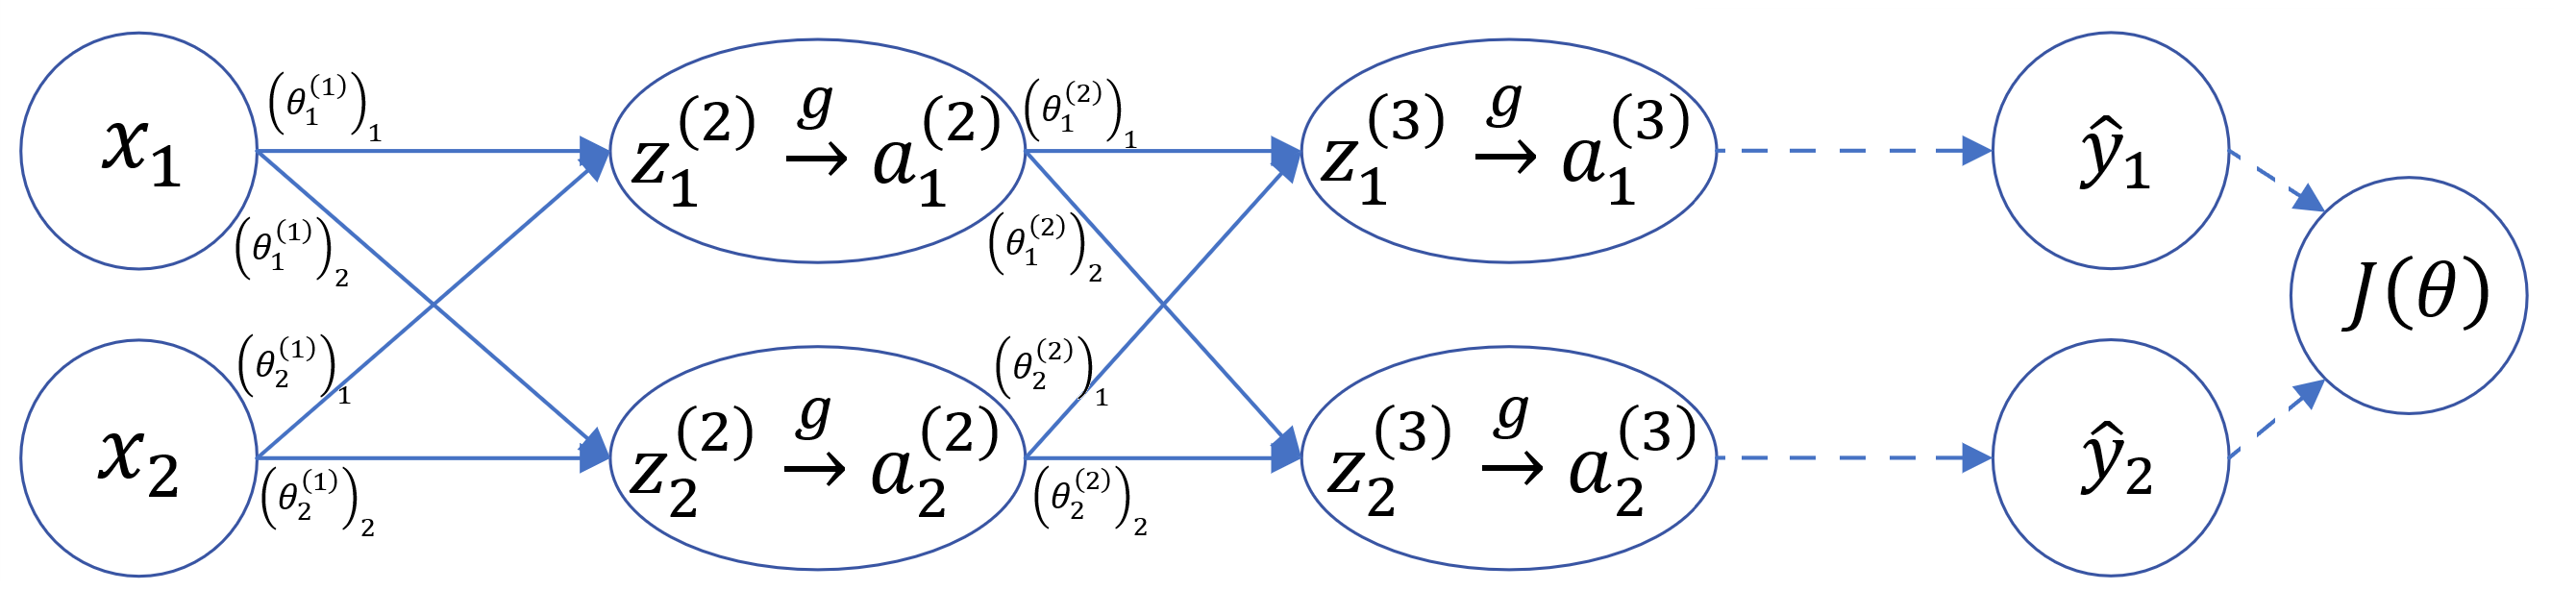
\includegraphics[width=\linewidth]{1}
    \caption{反向传播符号含义图示}
\end{figure}

如图1(省略了偏置),输入数据为$x=\begin{bmatrix}x_1\\x_2\end{bmatrix}$,实际输出为$y=\begin{bmatrix}y_1\\y_2\end{bmatrix}$

这张图上画出了所有运算,例如:

\[a_1^{\left(2\right)}=g\left(z_1^{\left(2\right)}\right)\]

\[z_2^{\left(2\right)}=\left(\theta_1^{\left(1\right)}\right)_1x_1+\left(\theta_1^{\left(1\right)}\right)_2x_2\]

同时,此图认为预测输出为$\hat y_1=a_1^{\left(3\right)}$,即有误差(注意此处不是定义而是结论):

\[\delta_1^{\left(3\right)}=\hat y_1-y_1=a_1^{\left(3\right)}-y_1\]

\subsubsection{推导}

下面我们将上列函数改写成对应元素的写法,先作定义:

\begin{definition}[字母定义]
    字母$L,m,n$

    $L$:被$\theta$作用的层

    $m$:$L$层单元数量,用$j$进行遍历(即$j\in\left\{1,2,\cdots,m\right\}$)

    $n$:$L$层单元数量,用$i$进行遍历
\end{definition}

综上可得,若L是倒数第二层,则有:

\begin{corollary}[误差$\delta$定义]
    \[\begin{aligned}
            \delta_i^{\left(L+1\right)}
             & =\frac{\partial J}{\partial z_i^{\left(L+1\right)}}                                      \\
             & =\frac{\partial J}{\partial a_i^{\left(L+1\right)}}
             &
             & \cdot\frac{\partial a_i^{\left(L+1\right)}}{\partial z_i^{\left(L+1\right)}}             \\
             & =\left(\frac{-y_i}{a_i^{\left(L+1\right)}}+\frac{1-y_i}{1-a_i^{\left(L+1\right)}}\right)
             &
             & \cdot g^\prime z_i^{\left(L+1\right)}                                                    \\
             & =\left(\frac{-y_i}{a_i^{\left(L+1\right)}}+\frac{1-y_i}{1-a_i^{\left(L+1\right)}}\right)
             &
             & \cdot a_i^{\left(L+1\right)}\left(1-a_i^{\left(L+1\right)}\right)                        \\
             & =a_i^{\left(L+1\right)}-y_i
        \end{aligned}\]
\end{corollary}

将同一层$\delta^{\left(L+1\right)}$合并为矩阵得$\delta,a,y$都是列向量):

\[\delta^{\left(L+1\right)}=a^{\left(L+1\right)}-y\]

下面推隐含层,以第一个单元为例:

\[\begin{aligned}
        \delta_1^{\left(2\right)}
         & =\frac{\partial J}{\partial z_1^{\left(2\right)}}                        \\
         & =\frac{\partial J}{\partial z_1^{\left(3\right)}}
         &
         & \cdot\frac{\partial z_1^{\left(3\right)}}{\partial a_1^{\left(2\right)}}
         &
         & \cdot\frac{\partial a_1^{\left(2\right)}}{\partial z_1^{\left(2\right)}}
         &
         & +\frac{\partial J}{\partial z_2^{\left(3\right)}}
         &
         & \cdot\frac{\partial z_2^{\left(3\right)}}{\partial a_1^{\left(2\right)}}
         &
         & \cdot\frac{\partial a_1^{\left(2\right)}}{\partial z_1^{\left(2\right)}} \\
         & =\delta_1^{\left(3\right)}
         &
         & \cdot\left(\theta_1^{\left(2\right)}\right)_1
         &
         & \cdot g^\prime z_1^{\left(2\right)}
         &
         & +\delta_2^{\left(3\right)}
         &
         & \cdot\left(\theta_1^{\left(2\right)}\right)_2
         &
         &
        \cdot g^\prime z_1^{\left(2\right)}
    \end{aligned}\]

令:

\[\left\{\begin{aligned}
        \delta^{\left(L\right)}   & =\begin{bmatrix}\delta_1^{\left(L\right)}\\\delta_2^{\left(L\right)}\\\vdots\\\delta_n^{\left(L\right)}\end{bmatrix} \\
        \theta_i^{\left(L\right)} & =\begin{bmatrix}
                                         \left(\theta_i^{\left(L\right)}\right)_1 &
                                         \left(\theta_i^{\left(L\right)}\right)_2 &
                                         \cdots                                   &
                                         \left(\theta_i^{\left(L\right)}\right)_n
                                     \end{bmatrix}\end{aligned}\right.\]

可将上式化为矩阵:

\[\delta_1^{\left(2\right)}
    =\theta_1^{\left(2\right)}\delta^{\left(3\right)}
    \cdot g^\prime z_1^{\left(2\right)}\]

\subsubsection{结论}

由上,可写出递推普式:

\[\delta_j^{\left(L\right)}
    =\theta_j^{\left(L\right)}\delta^{\left(L+1\right)}\cdot g^\prime z_j^{\left(L\right)}\]

其中最后一层:

\[\delta^{\left(Last\right)}=a^{\left(Last\right)}-y\]

\newpage
\part{实矩阵的三个等价关系}

\section{矩阵的等价}

\begin{definition}[行等价、列等价和等价]
    \[\begin{aligned}
            A,B\text{行等价} & \iff PA=B  \\
            A,B\text{列等价} & \iff AQ=B  \\
            A,B\text{等价}   & \iff PAQ=B
        \end{aligned}\]    其中:
    \[\begin{aligned}
            A                     & =A_{m,n} \\
            B                     & =B_{m,n} \\
            R\left(P_{m,m}\right) & =m       \\
            R\left(Q_{n,n}\right) & =n
        \end{aligned}\]\end{definition}

\begin{theorem}[反身性]
    \[A,A\text{等价}\]
\end{theorem}

\begin{proof}
    \[\begin{aligned}
                     & EAE=A          \\
            \implies & A,A\text{等价}
        \end{aligned}\]\end{proof}

\begin{theorem}[对称性]
    \[A,B\text{等价}\implies B,A\text{等价}\]
\end{theorem}

\begin{proof}
    \[\begin{aligned}
                     & R\left(P\right)=m,R\left(Q\right)=n \\
            \implies & \exists P^{-1},Q^{-1}               \\
            \implies & P^{-1}BQ^{-1}=A                     \\
            \implies & B,A\text{等价}
        \end{aligned}\]\end{proof}

\begin{theorem}[传递性]
    \[A,B\text{等价},B,C\text{等价}
        \implies A,C\text{等价}\]
\end{theorem}

\begin{proof}
    \[\begin{aligned}
                     & A,B\text{等价},B,C\text{等价}                                 \\
            \implies & P_1AQ_1=B,P_2BQ_2=C                                           \\
            \implies & P_2^{-1}\left(P_1^{-1}AQ_1^{-1}\right)Q_2^{-1}=C              \\
            \implies & \left(P_2^{-1}P_1^{-1}\right)A\left(Q_1^{-1}Q_2^{-1}\right)=C \\
            \implies & A,C\text{等价}
        \end{aligned}\]\end{proof}

\subsection{等价在生活、数学的运用}

\subsubsection{增广矩阵解线性方程组}

若有线性方程组:

\[\left\{\begin{aligned}
        \sum_i a_{1i}x_i & =b_1 \\
        \sum_i a_{2i}x_i & =b_2 \\
        \vdots                  \\
        \sum_i a_{mi}x_i & =b_m
    \end{aligned}\right.\]

则对应增广矩阵

\[\begin{bmatrix}
        a_{11} & a_{12} & \cdots & a_{1n} & b_1    \\
        a_{21} & a_{22} & \cdots & a_{2n} & b_2    \\
        \vdots & \vdots & \ddots & \vdots & \vdots \\
        a_{m1} & a_{m2} & \cdots & a_{mn} & b_m    \\
    \end{bmatrix}\]

经过任意初等行变换之后,仍可以表示为原方程组。

\subsection{实矩阵等价关系下的不变量}

\begin{theorem}[等价矩阵秩相同]
    \[A,B\text{等价}\implies R\left(A\right)=R\left(B\right)\]
\end{theorem}

\subsection{矩阵等价的充分必要条件}

\begin{theorem}[矩阵等价的充要条件是同秩]
    \[A,B\text{等价}\iff R\left(A\right)=R\left(B\right)\]
\end{theorem}

\begin{proof}
    在$A,B$同型前提下:

    将$A,B$化为标准型:

    \[\left\{\begin{aligned}
            A & =P_1D_1Q_1 =
            \begin{bmatrix}
                E_A & O \\
                O   & O
            \end{bmatrix}   \\
            B & =P_2D_2Q_2 =
            \begin{bmatrix}
                E_B & O \\
                O   & O
            \end{bmatrix}
        \end{aligned}\right.\]

    充分性:$A,B\text{等价}\impliedby R\left(A\right)=R\left(B\right)$
    \[\begin{aligned}
                      & R\left(A\right)=R\left(B\right)=k \\
            \implies  & D_1=D_2
            \\
            \text{取} & P=P_2P_1^{-1},Q=Q_1^{-1}Q_2       \\
            \implies  & PAQ=B                             \\
            \implies  & A,B\text{等价}
        \end{aligned}\]

    必要性:$A,B\text{等价}\implies R\left(A\right)=R\left(B\right)$
    \[\begin{aligned}
                     & A,B\text{等价}                          \\
            \implies & PAQ=B                                   \\
            \implies & P\left(P_1D_1Q_1\right)Q=B              \\
            \implies & \left(PP_1\right)D_1\left(Q_1Q\right)=B \\
            \implies & R\left(A\right)=R\left(D_1\right)=
            R\left(B\right)\left(=R\left(D_2\right)\right)
        \end{aligned}\]
\end{proof}

\subsection{等价标准形化的方法}

\begin{theorem}[初等变换]

    矩阵初等变换后与之前等价

    行:$r_i$,列:$c_i$

    \begin{enumerate}
        \item 对换两行(列):$r_i\leftrightarrow r_j$
        \item $k$乘某行(列):$kr_i$或$r_i\times k\left(k\neq0\right)$
        \item 加某行(列)$k$倍:$r_i+kr_j$
    \end{enumerate}
\end{theorem}

\section{方阵的相似}

\begin{definition}[相似]
    \[A\sim B\iff P^{-1}AP=B\]
\end{definition}

\begin{theorem}[反身性]
    \[A\sim A\]
\end{theorem}

\begin{theorem}[对称性]
    \[A\sim B\implies B\sim A\]
\end{theorem}

\begin{theorem}[传递性]
    \[A\sim B, B\sim C\implies A\sim C\]
\end{theorem}

\subsection{实方阵相似关系下的不变量}

\begin{theorem}[相似方阵特征多项式相同]
    \[A\sim B\implies\det\left(A-\lambda_A E\right)=\det\left(B-\lambda_B E\right)\]
\end{theorem}

\begin{corollary}[相似方阵特征值相同]
    \[A\sim B\implies\lambda_A=\lambda_B\]
\end{corollary}

\begin{corollary}[相似方阵迹相同]
    \[A\sim B\implies{\rm tr}A={\rm tr}B\]
\end{corollary}

\begin{proof}
    \[\begin{aligned}
                     & A\sim B                                                 \\
            \implies & P^{-1}AP=B                                              \\
            \implies & \det\left(B-\lambda E\right)                            \\
            =        & \det\left(P^{-1}AP-\lambda P^{-1}EP\right)              \\
            =        & \det\left(P^{-1}\left(A-\lambda E\right)P\right)        \\
            =        & \det P^{-1}\cdot\det\left(A-\lambda E\right)\cdot\det P \\
            =        & \det\left(A-\lambda E\right)
        \end{aligned}\]
\end{proof}

\begin{theorem}[相似方阵行列式相同]
    \[A\sim B\implies\det A=\det B\]
\end{theorem}

\begin{proof}
    \[\begin{aligned}
                     & A\sim B                                   \\
            \implies & P^{-1}AP=B                                \\
            \implies & \det\left(P^{-1}AP\right)=\det B          \\
            \implies & \det P^{-1}\cdot\det A\cdot\det P =\det B \\
            \implies & \det A=\det B                             \\
            \implies & \lambda A=\lambda B                       \\
                     & {\rm tr}A={\rm tr}B
        \end{aligned}\]
\end{proof}

\begin{theorem}[相似方阵等价]
    \[A\sim B\implies A,B\text{等价}\]
\end{theorem}

\begin{corollary}[相似方阵秩相同]
    \[A\sim B\implies R\left(A\right)=R\left(B\right)\]
\end{corollary}

\begin{proof}
    \[\begin{aligned}
                     & A\sim B                         \\
            \implies & P^{-1}AP=B                      \\
                     & P,P^{-1}\text{满秩}             \\
            \implies & A,B\text{等价}                  \\
            \implies & R\left(A\right)=R\left(B\right)
        \end{aligned}\]
\end{proof}

\begin{corollary}[相似方阵逆也相似(如果有逆)]
    \[A\sim B,\exists A^{-1},B^{-1}\implies A^{-1}\sim B^{-1}\]
\end{corollary}

\begin{proof}
    \[\begin{aligned}
                     & \exists A^{-1},B^{-1}      \\
            \implies & B^{-1}                     \\
            =        & \left(P^{-1}AP\right)^{-1} \\
            =        & PA^{-1}P^{-1}              \\
            \implies & A^{-1}\sim B^{-1}
        \end{aligned}\]
\end{proof}

\section{方阵的可对角化}

\begin{definition}[可对角化]
    \[A_n\sim\Lambda\]
\end{definition}

\begin{corollary}[对角矩阵$\Lambda$和特征向量$\vec{\rm p}$、矩阵$P$]
    \[\def \p {\vec{\rm p}}
        A\sim\Lambda\implies P^{-1}AP=\Lambda
        \left\{\begin{aligned}
            \Lambda & =
            \begin{bmatrix}
                \lambda_1 &           &        &           \\
                          & \lambda_2 &        &           \\
                          &           & \ddots &           \\
                          &           &        & \lambda_n
            \end{bmatrix}                   \\
            P       & =\begin{bmatrix}\p_1&\p_2&\cdots&\p_n\end{bmatrix}
        \end{aligned}\right.\]
\end{corollary}\label{corollary5.0.0.1}

\subsection{方阵可对角化的充分必要条件}

\begin{theorem}[方阵可对角化充要条件是$A$有$n$个线性无关特征向量]
    \[A\sim\Lambda\iff\text{全体线性无关}\vec{\rm p}\text{数}=n\]

    若设$r=\lambda$重数,

    又$R\left(A-\lambda E\right)=\lambda$对应线性无关${\vec{\rm p}}$数,

    即:

    \[A\sim\Lambda\iff R\left(A-\lambda E\right)=n-r\]
\end{theorem}

\begin{proof}
    \cite{4}由\ref{corollary5.0.0.1}定义

    充分性:$A\sim\Lambda\impliedby\text{全体线性无关}\vec{\rm p}\text{数}=n$

    \[\def \p {\vec{\rm p}}
        \begin{aligned}
            AP
            =         & \begin{bmatrix}A\p_1 & A\p_2 & \cdots & A\p_n\end{bmatrix}                         \\
            =         & \begin{bmatrix}\lambda_1\p_1 & \lambda_2\p_2 & \cdots & \lambda_n\p_n\end{bmatrix} \\
            =         & \begin{bmatrix}
                            \lambda_1 &           &        &           \\
                                      & \lambda_2 &        &           \\
                                      &           & \ddots &           \\
                                      &           &        & \lambda_n
                        \end{bmatrix}
            \begin{bmatrix}\p_1&\p_2&\cdots&\p_n\end{bmatrix}                                              \\
            =         & \Lambda P                                                                          \\
            \text{又} & \begin{bmatrix}\p_1&\p_2&\cdots&\p_n\end{bmatrix}\text{线性无关}                   \\
            \implies  & \exists P^{-1}                                                                     \\
            \implies  & P^{-1}AP=\Lambda                                                                   \\
            \implies  & A\sim\Lambda
        \end{aligned}\]

    必要性:$A\sim\Lambda\implies\text{全体线性无关}\vec{\rm p}\text{数}=n$
    \[\def \p {\vec{\rm p}}
        \begin{aligned}
            A\sim\Lambda
            \implies  & AP=\Lambda P                                                                                    \\
            \implies  & AP=\begin{bmatrix}A\p_1 & A\p_2 & \cdots & A\p_n\end{bmatrix}                                   \\
            =         & \Lambda P=\begin{bmatrix}\lambda_1\p_1 & \lambda_2\p_2 & \cdots & \lambda_n\p_n\end{bmatrix}    \\
            \text{又} & \exists P^{-1}                                                                                  \\
            \implies  & \begin{bmatrix}\p_1&\p_2&\cdots&\p_n\end{bmatrix}\text{线性无关且为特征向量}                    \\
                      & \begin{bmatrix}\lambda_1 & \lambda_2 & \ddots & \lambda_n\end{bmatrix}\text{是}A\text{的特征值}
        \end{aligned}\]
\end{proof}

\subsection{对角化的方法}

\begin{theorem}[特征多项式]
    令特征多项式值为$0$,解得$\lambda$值即为特征值,根重数为对应特征值重数

    \[\det\left(A-\lambda E\right)=
        \begin{vmatrix}
            a_{11}-\lambda & a_{12}         & \cdots & a_{1n}         \\
            a_{21}         & a_{22}-\lambda & \cdots & a_{2n}         \\
            \vdots         & \vdots         & \ddots & \vdots         \\
            a_{m1}         & a_{m2}         & \cdots & a_{mn}-\lambda \\
        \end{vmatrix}\]
\end{theorem}

\section{方阵的合同}

\begin{definition}[合同]
    \[A,B\text{合同}\iff B=C^TAC,\exists C^{-1}\]
\end{definition}

\begin{theorem}[反身性]
    \[A,A\text{合同}\]
\end{theorem}

\begin{theorem}[对称性]
    \[A,B\text{合同}\implies B,A\text{合同}\]
\end{theorem}

\begin{theorem}[传递性]
    \[A,B\text{合同},B,C\text{合同}\implies A,C\text{合同}\]
\end{theorem}

\subsection{实对称方阵合同关系下的不变量}

\begin{theorem}[合同方阵都是对称矩阵]
    \[A,B\text{合同}\implies B=B^T\]
\end{theorem}

\begin{corollary}[合同方阵秩相同]
    \[A,B\text{合同}\implies R\left(A\right)=R\left(B\right)\]
\end{corollary}

\begin{proof}
    \[\begin{aligned}
                      & A,B\text{合同}
            \implies  & B=C^TAC                         \\
            \implies  & B^T=\left(C^TAC\right)^T        \\
            =         & C^TA^TC                         \\
            =         & B                               \\
            \text{又} & \exists C^{-1}                  \\
            \implies  & A,B\text{等价}                  \\
            \implies  & R\left(A\right)=R\left(B\right)
        \end{aligned}\]
\end{proof}

\begin{theorem}[合同方阵惯性指数相同]
    \[A,B,C\text{合同}\implies A,B\text{正负惯性指数相同}\]
\end{theorem}

\subsection{实对称方阵合同的充分必要条件}

\begin{theorem}
    \[A,B\text{合同}\iff\text{实对称方阵}A,B\text{正负惯性指数相同}\]
\end{theorem}

\subsection{标准形化的方法}

\begin{theorem}[正交变换法]
    \[\text{二次型}A\to\text{标准型}B\]

    1. 令$\det\left(A-\lambda E\right)=0$,解得$n$个特征值$\{\lambda_n\}$

    2. 令$\left(A-\lambda_iE\right)\vec{\rm p}=\vec 0$,解得线性无关特征向量组$\{\vec{\rm p}_n\}$

    3. 用格拉姆-施密特正交单位化,解得正交单位特征向量组$\{\vec{\rm e}_n\}$

    4. 用正交单位特征向量组构建正交矩阵$\def \e {\vec{\rm e}}
        P=\begin{bmatrix}\e_1&\e_2&\cdots&\e_n\end{bmatrix}$

    5. $\vec{\rm x}=P\vec{\rm y}$即可将$A$化为标准型$B$
\end{theorem}

\newpage
\part{本课程的学习体会}

\paragraph{}
在每次提出新概念的时候我都很难理解,只能靠后续学习或者多做题巩固。在学习行列式的时候,通过平行四边形、平行六面体等概念理解了一些。但后续更多知识点也许需要更高阶的知识才能感性理解,让我意识到总是寻求感性理解是不现实的。尤其工科更重视运用的学科更难刨根问底。

\paragraph{}
我学习的时候还养成了看完定理喜欢阅读证明的习惯,虽然可以增强理解,但会很耗精力。尤其是有些定理的良定义也许要到更高阶的学习后才能理解。一味寻求理解并不现实,还是要循序渐进才行。

\paragraph{}
在学习过程中经常遇到的问题是初等教育和大学、大学学科之间数学符号冲突让我很头疼,希望能有统一的标准,方便查阅使用。还有又许多常用的定理会以例题的形式出现在课本中,查询十分麻烦,如果可以将定理、证明和例题分列几处就更好了。

\newpage
\begin{thebibliography}{99}
    \bibitem{1} Wikipedia. Linear Algebra: History.
    \bibitem{2} [美] 吴恩达. Machine Learning.
    \bibitem{3} [美] Sheldon Axler. Linear Algebra Done Right [M]. 北京: 人民邮电出版社, 1996.
    \bibitem{4} [美] David C.Lay. Linear Algebra and Its Applications [M]. 北京: 机械工业出版社, 2005.
    \bibitem{5} 唐烁, 朱士信. 线性代数 [M]. 北京: 机械工业出版社, 2018.
\end{thebibliography}

\begin{appendix}
    \section{附录1}

    \href{https://github.com/Poker-sang/Notes}{https://github.com/Poker-sang/Notes}

    \href{https://www.bilibili.com/read/cv16091164}{https://www.bilibili.com/read/cv16091164}
\end{appendix}

\end{document}